\documentclass{article}
\usepackage{fancyhdr} % Required for custom headers
\usepackage{lastpage} % Required to determine the last page for the footer
\usepackage{extramarks} % Required for headers and footers
\usepackage[usenames,dvipsnames]{color} % Required for custom colors
\usepackage{graphicx} % Required to insert images
\usepackage{listings} % Required for insertion of code
\usepackage{courier} % Required for the courier font
\usepackage{lipsum} % Used for inserting dummy 'Lorem ipsum' text into the template
\usepackage{caption}
\usepackage{subcaption}
\usepackage{amsmath}
\usepackage{amsfonts}
\usepackage{amssymb}
\usepackage{epstopdf}
\usepackage{placeins}
\usepackage{color} 
\usepackage{fancyvrb} 
\usepackage{setspace}
\usepackage[numbered]{bookmark}
\usepackage{tikz}
\usepackage{pgfplots}
\usepackage[absolute,overlay]{textpos}
\usetikzlibrary{calc}
\usetikzlibrary{pgfplots.fillbetween, backgrounds}
\usetikzlibrary{positioning}
\usetikzlibrary{arrows}
\usetikzlibrary{pgfplots.groupplots}
\usetikzlibrary{arrows.meta}
\usetikzlibrary{plotmarks}

\usepgfplotslibrary{groupplots}
\pgfplotsset{compat=newest} 
%\pgfplotsset{plot coordinates/math parser=false}
\DeclareGraphicsExtensions{.pdf,.png,.jpg}
\graphicspath{{figs/}}


\DeclareMathOperator{\E}{\mathbb{E}}
\newcommand{\Conv}{\mathop{\scalebox{1.5}{\raisebox{-0.2ex}{$\ast$}}}}%


% rect results in 1 if a < x < b, and 0 otherwise
\pgfmathdeclarefunction{rect}{3}{%
	\pgfmathparse{(and(#1 >= #2, #1 <= #3) * 1.0}%
}

\pgfplotsset{
	dirac/.style={
		mark=triangle*,
		mark options={scale=2},
		ycomb,
		scatter,
		visualization depends on={y/abs(y)-1 \as \sign},
		scatter/@pre marker code/.code={\scope[rotate=90*\sign,yshift=-2pt]}
	}
}

% Margins
\topmargin=-0.45in
\evensidemargin=0in
\oddsidemargin=0in
\textwidth=6.5in
\textheight=9.0in
\headsep=0.25in

\linespread{1.2} % Line spacing

% Set up the header and footer
\pagestyle{fancy}
\lhead{\hmwkAuthorName} % Top left header
\chead{\hmwkTitle} % Top center head
\rhead{\hmwkClass} % Top right header
\lfoot{} % Bottom left footer
\cfoot{} % Bottom center footer
\rfoot{Page\ \thepage\ of\ \protect\pageref{LastPage}} % Bottom right footer
\renewcommand\headrulewidth{0.4pt} % Size of the header rule
\renewcommand\footrulewidth{0.4pt} % Size of the footer rule

%\setlength\parindent{0pt} % Removes all indentation from paragraphs
\definecolor{MyDarkGreen}{rgb}{0.0,0.4,0.0} % This is the color used for comments
\lstloadlanguages{Perl} % Load Perl syntax for listings, for a list of other languages supported see: ftp://ftp.tex.ac.uk/tex-archive/macros/latex/contrib/listings/listings.pdf
\lstset{language=Perl, % Use Perl in this example
        frame=single, % Single frame around code
        basicstyle=\small\ttfamily, % Use small true type font
        keywordstyle=[1]\color{Blue}\bf, % Perl functions bold and blue
        keywordstyle=[2]\color{Purple}, % Perl function arguments purple
        keywordstyle=[3]\color{Blue}\underbar, % Custom functions underlined and blue
        identifierstyle=, % Nothing special about identifiers                                         
        commentstyle=\usefont{T1}{pcr}{m}{sl}\color{MyDarkGreen}\small, % Comments small dark green courier font
        stringstyle=\color{Purple}, % Strings are purple
        showstringspaces=false, % Don't put marks in string spaces
        tabsize=5, % 5 spaces per tab
        %
        % Put standard Perl functions not included in the default language here
        morekeywords={rand},
        %
        % Put Perl function parameters here
        morekeywords=[2]{on, off, interp},
        %
        % Put user defined functions here
        morekeywords=[3]{test},
       	%
        morecomment=[l][\color{Blue}]{...}, % Line continuation (...) like blue comment
        numbers=left, % Line numbers on left
        firstnumber=1, % Line numbers start with line 1
        numberstyle=\tiny\color{Blue}, % Line numbers are blue and small
        stepnumber=5 % Line numbers go in steps of 5
}

% Creates a new command to include a perl script, the first parameter is the filename of the script (without .pl), the second parameter is the caption
\newcommand{\perlscript}[2]{
\begin{itemize}
\item[]\lstinputlisting[caption=#2,label=#1]{#1.pl}
\end{itemize}
}

% Header and footer for when a page split occurs within a problem environment
\newcommand{\enterProblemHeader}[1]{
\nobreak\extramarks{#1}{#1 continued on next page\ldots}\nobreak
\nobreak\extramarks{#1 (continued)}{#1 continued on next page\ldots}\nobreak
}

% Header and footer for when a page split occurs between problem environments
\newcommand{\exitProblemHeader}[1]{
\nobreak\extramarks{#1 (continued)}{#1 continued on next page\ldots}\nobreak
\nobreak\extramarks{#1}{}\nobreak
}

\setcounter{secnumdepth}{0} % Removes default section numbers
\newcounter{homeworkProblemCounter} % Creates a counter to keep track of the number of problems

\newcommand{\homeworkProblemName}{}
\newenvironment{homeworkProblem}[1][Problem \arabic{homeworkProblemCounter}]{ % Makes a new environment called homeworkProblem which takes 1 argument (custom name) but the default is "Problem #"
\stepcounter{homeworkProblemCounter} % Increase counter for number of problems
\renewcommand{\homeworkProblemName}{#1} % Assign \homeworkProblemName the name of the problem
\section{\homeworkProblemName} % Make a section in the document with the custom problem count
\enterProblemHeader{\homeworkProblemName} % Header and footer within the environment
}{
\exitProblemHeader{\homeworkProblemName} % Header and footer after the environment
}

\newcommand{\problemAnswer}[1]{ % Defines the problem answer command with the content as the only argument
\noindent\framebox[\columnwidth][c]{\begin{minipage}{0.98\columnwidth}#1\end{minipage}} % Makes the box around the problem answer and puts the content inside
}

\newcommand{\homeworkSectionName}{}
\newenvironment{homeworkSection}[1]{ % New environment for sections within homework problems, takes 1 argument - the name of the section
\renewcommand{\homeworkSectionName}{#1} % Assign \homeworkSectionName to the name of the section from the environment argument
\subsection{\homeworkSectionName} % Make a subsection with the custom name of the subsection
\enterProblemHeader{\homeworkProblemName\ [\homeworkSectionName]} % Header and footer within the environment
}{
\enterProblemHeader{\homeworkProblemName} % Header and footer after the environment
}

%----------------------------------------------------------------------------------------
%	NAME AND CLASS SECTION
%----------------------------------------------------------------------------------------
%%%%%%%%%%%%%%%%%%%%%%%%%%%%%%%%%%%%%%%%%%%%%%%%%%%%%%%%%%%%%%%%%%%%%%%%%%%%%%%%%%%%%%%%%
\newcommand{\hmwkTitle}{Homework \#04} % Assignment title
\newcommand{\hmwkDueDate}{\today} % Due date
\newcommand{\hmwkClass}{EE 264 (Summer 2018)} % Course/class
\newcommand{\hmwkAuthorName}{Solutions} % Your name
%%%%%%%%%%%%%%%%%%%%%%%%%%%%%%%%%%%%%%%%%%%%%%%%%%%%%%%%%%%%%%%%%%%%%%%%%%%%%%%%%%%%%%%%%
%----------------------------------------------------------------------------------------
%	TITLE PAGE
%----------------------------------------------------------------------------------------
\title{
\vspace{2in}
\textmd{\textbf{\hmwkClass:\ \hmwkTitle}}\\
\normalsize\vspace{0.1in}\small{Due\ on\ \hmwkDueDate}\\
\vspace{0.1in}\large{\textit{\hmwkClassInstructor\ \hmwkClassTime}}
\vspace{3in}
}

\author{\textbf{\hmwkAuthorName}}
\date{} % Insert date here if you want it to appear below your name

%----------------------------------------------------------------------------------------

\begin{document}
\section{Problem 1}
\subsection{(a)}
\resizebox{\linewidth}{!}{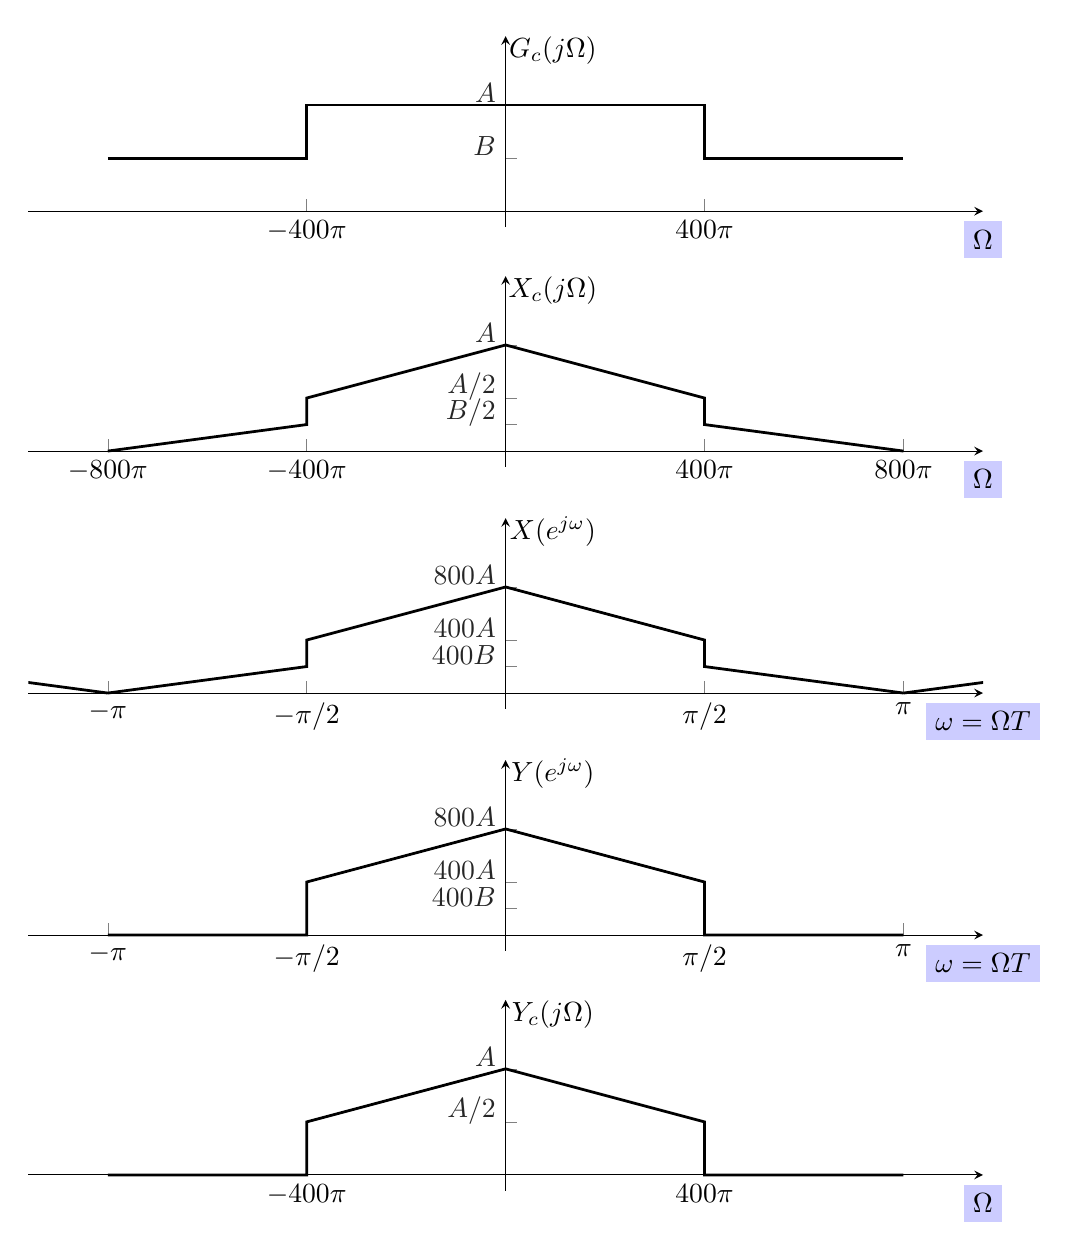
\begin{tikzpicture}
\begin{axis}[
	name=plot1,
	axis lines*=middle,
	enlargelimits = true,
	clip=true,
	scale only axis,
	width=\textwidth,
	height=0.2\textwidth,
	ymin=0, ymax=3,
	xmin=-8, xmax=8,
	axis line style={->,>=stealth},
	xlabel={\tikz[baseline]{\node[fill=blue!20,anchor=base] (t1) {$\Omega$};}},
	ylabel={$G_c(j\Omega)$},
	every axis x label/.style={
		at={(ticklabel* cs:1)},
		%xshift=0.2cm,
		anchor=north,
	},
	every axis y label/.style={
		at={(ticklabel* cs:0.8)},
		anchor=south,
		xshift=0.6cm,
	},
	ytick={1, 2},
	yticklabels={$B$, $A$},
	yticklabel style={yshift=0.15cm},
	xtick={-4, 4},
	xticklabels={$-400\pi$, $400\pi$}, 
	every outer y axis line/.append style={white!15!black},
	every y tick label/.append style={font=\color{white!15!black}},
	legend style={draw=white!15!black,fill=white,legend cell align=left}]
	\addplot[solid, line width=1pt] coordinates {(-8, 1) (-4, 1) (-4, 2) (4, 2) (4, 1) (8, 1)};
\end{axis}

\begin{axis}[
name=plot2,
at=(plot1.below south east), anchor=above north east,
axis lines*=middle,
enlargelimits = true,
clip=true,
scale only axis,
width=\textwidth,
height=0.2\textwidth,
ymin=0, ymax=3,
xmin=-8, xmax=8,
axis line style={->,>=stealth},
xlabel={\tikz[baseline]{\node[fill=blue!20,anchor=base] (t1) {$\Omega$};}},
ylabel={$X_c(j\Omega)$},
every axis x label/.style={
	at={(ticklabel* cs:1)},
	%xshift=0.2cm,
	anchor=north,
},
every axis y label/.style={
	at={(ticklabel* cs:0.8)},
	anchor=south,
	xshift=0.6cm,
},
ytick={0.5, 1, 2},
yticklabels={$B/2$, $A/2$, $A$},
yticklabel style={yshift=0.15cm},
xtick={-8, -4, 4, 8},
xticklabels={$-800\pi$, $-400\pi$, $400\pi$, $800\pi$}, 
every outer y axis line/.append style={white!15!black},
every y tick label/.append style={font=\color{white!15!black}},
legend style={draw=white!15!black,fill=white,legend cell align=left}]
\addplot[solid, line width=1pt] coordinates {(-8, 0) (-4, 1/2) (-4, 1) (0, 2) (4, 1) (4, 1/2) (8, 0)};
\end{axis}

\begin{axis}[
name=plot3,
at=(plot2.below south east), anchor=above north east,
axis lines*=middle,
enlargelimits = true,
clip=true,
scale only axis,
width=\textwidth,
height=0.2\textwidth,
ymin=0, ymax=3,
xmin=-8, xmax=8,
axis line style={->,>=stealth},
xlabel={\tikz[baseline]{\node[fill=blue!20,anchor=base] (t1) {$\omega = \Omega T$};}},
ylabel={$X(e^{j\omega})$},
every axis x label/.style={
	at={(ticklabel* cs:1)},
	%xshift=0.2cm,
	anchor=north,
},
every axis y label/.style={
	at={(ticklabel* cs:0.8)},
	anchor=south,
	xshift=0.6cm,
},
ytick={0.5, 1, 2},
yticklabels={$400B$, $400A$, $800A$},
yticklabel style={yshift=0.15cm},
xtick={-8, -4, 4, 8},
xticklabels={$-\pi$, $-\pi/2$, $\pi/2$, $\pi$}, 
every outer y axis line/.append style={white!15!black},
every y tick label/.append style={font=\color{white!15!black}},
legend style={draw=white!15!black,fill=white,legend cell align=left}]
\addplot[solid, line width=1pt] coordinates {(-8, 0) (-4, 1/2) (-4, 1) (0, 2) (4, 1) (4, 1/2) (8, 0)};
\addplot[solid, line width=1pt] coordinates {(-8+16, 0) (-4+16, 1/2) (-4+16, 1) (0+16, 2) (4+16, 1) (4+16, 1/2) (8+16, 0)};
\addplot[solid, line width=1pt] coordinates {(-8-16, 0) (-4-16, 1/2) (-4-16, 1) (0-16, 2) (4-16, 1) (4-16, 1/2) (8-16, 0)};
\end{axis}

\begin{axis}[
name=plot4,
at=(plot3.below south east), anchor=above north east,
axis lines*=middle,
enlargelimits = true,
clip=true,
scale only axis,
width=\textwidth,
height=0.2\textwidth,
ymin=0, ymax=3,
xmin=-8, xmax=8,
axis line style={->,>=stealth},
xlabel={\tikz[baseline]{\node[fill=blue!20,anchor=base] (t1) {$\omega = \Omega T$};}},
ylabel={$Y(e^{j\omega})$},
every axis x label/.style={
	at={(ticklabel* cs:1)},
	%xshift=0.2cm,
	anchor=north,
},
every axis y label/.style={
	at={(ticklabel* cs:0.8)},
	anchor=south,
	xshift=0.6cm,
},
ytick={0.5, 1, 2},
yticklabels={$400B$, $400A$, $800A$},
yticklabel style={yshift=0.15cm},
xtick={-8, -4, 4, 8},
xticklabels={$-\pi$, $-\pi/2$, $\pi/2$, $\pi$}, 
every outer y axis line/.append style={white!15!black},
every y tick label/.append style={font=\color{white!15!black}},
legend style={draw=white!15!black,fill=white,legend cell align=left}]
\addplot[solid, line width=1pt] coordinates {(-8, 0) (-4, 0) (-4, 1) (0, 2) (4, 1) (4, 0) (8, 0)};
\end{axis}

\begin{axis}[
name=plot5,
at=(plot4.below south east), anchor=above north east,
axis lines*=middle,
enlargelimits = true,
clip=true,
scale only axis,
width=\textwidth,
height=0.2\textwidth,
ymin=0, ymax=3,
xmin=-8, xmax=8,
axis line style={->,>=stealth},
xlabel={\tikz[baseline]{\node[fill=blue!20,anchor=base] (t1) {$\Omega$};}},
ylabel={$Y_c(j\Omega)$},
every axis x label/.style={
	at={(ticklabel* cs:1)},
	%xshift=0.2cm,
	anchor=north,
},
every axis y label/.style={
	at={(ticklabel* cs:0.8)},
	anchor=south,
	xshift=0.6cm,
},
ytick={1, 2},
yticklabels={$A/2$, $A$},
yticklabel style={yshift=0.15cm},
xtick={-4, 4},
xticklabels={$-400\pi$, $400\pi$}, 
every outer y axis line/.append style={white!15!black},
every y tick label/.append style={font=\color{white!15!black}},
legend style={draw=white!15!black,fill=white,legend cell align=left}]
\addplot[solid, line width=1pt] coordinates {(-8, 0) (-4, 0) (-4, 1) (0, 2) (4, 1) (4, 0) (8, 0)};
\end{axis}

\end{tikzpicture}
}

\subsection{(b)}
We want to obtain $y_c(t) = f_c(t-0.1)$. In the frequency domain,

\begin{align}
Y_c(j\Omega) &= F_c(j\Omega)e^{-j0.1\Omega} \tag{Delay property of the Fourier transform} \\
Y(e^{j\omega}) &= F_c(j\omega/T)e^{-j0.1\omega/T} \tag{Since $\Omega = \omega/T$ and there is no aliasing} \\
Y(e^{j\omega}) &= F_c(j\omega/T)e^{-j80\omega} \tag{$T = 1/800$}
\end{align}

\resizebox{\linewidth}{!}{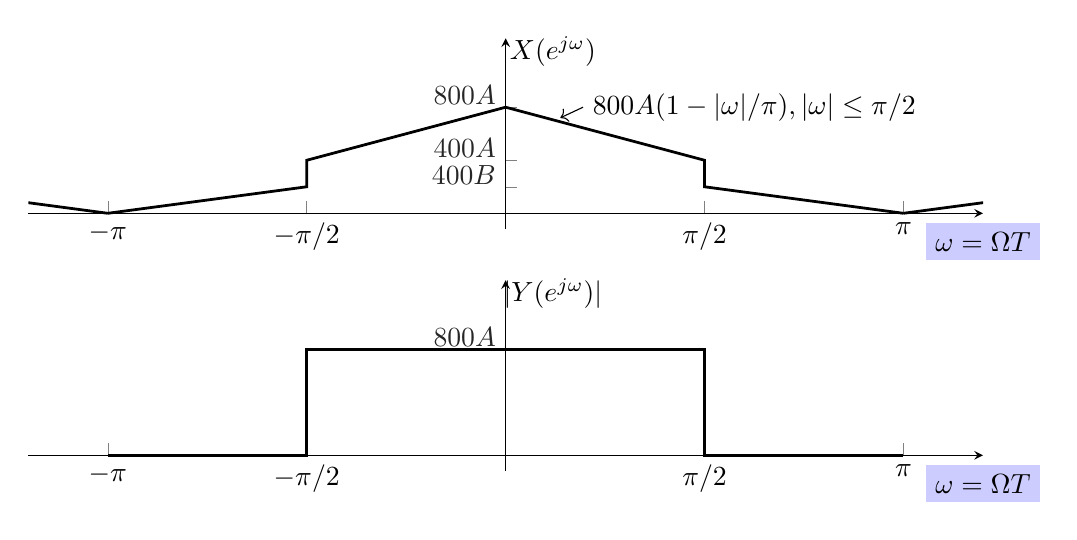
\begin{tikzpicture}
\begin{axis}[
	name=plot1,
	%at=(plot2.below south east), anchor=above north east,
	axis lines*=middle,
	enlargelimits = true,
	clip=true,
	scale only axis,
	width=\textwidth,
	height=0.2\textwidth,
	ymin=0, ymax=3,
	xmin=-8, xmax=8,
	axis line style={->,>=stealth},
	xlabel={\tikz[baseline]{\node[fill=blue!20,anchor=base] (t1) {$\omega = \Omega T$};}},
	ylabel={$X(e^{j\omega})$},
	every axis x label/.style={
		at={(ticklabel* cs:1)},
		%xshift=0.2cm,
		anchor=north,
	},
	every axis y label/.style={
		at={(ticklabel* cs:0.8)},
		anchor=south,
		xshift=0.6cm,
	},
	ytick={0.5, 1, 2},
	yticklabels={$400B$, $400A$, $800A$},
	yticklabel style={yshift=0.15cm},
	xtick={-8, -4, 4, 8},
	xticklabels={$-\pi$, $-\pi/2$, $\pi/2$, $\pi$}, 
	every outer y axis line/.append style={white!15!black},
	every y tick label/.append style={font=\color{white!15!black}},
	legend style={draw=white!15!black,fill=white,legend cell align=left}]
	\addplot[solid, line width=1pt] coordinates {(-8, 0) (-4, 1/2) (-4, 1) (0, 2) (4, 1) (4, 1/2) (8, 0)};
	\addplot[solid, line width=1pt] coordinates {(-8+16, 0) (-4+16, 1/2) (-4+16, 1) (0+16, 2) (4+16, 1) (4+16, 1/2) (8+16, 0)};
	\addplot[solid, line width=1pt] coordinates {(-8-16, 0) (-4-16, 1/2) (-4-16, 1) (0-16, 2) (4-16, 1) (4-16, 1/2) (8-16, 0)};
	\node (t1) at (axis cs: 5, 2) {$800A(1-|\omega|/\pi), |\omega|\leq\pi/2$};
	\draw[->] (t1.west) to (axis cs: 1.1, 1.8) {};
\end{axis}

\begin{axis}[
	name=plot2,
	at=(plot1.below south east), anchor=above north east,
	axis lines*=middle,
	enlargelimits = true,
	clip=true,
	scale only axis,
	width=\textwidth,
	height=0.2\textwidth,
	ymin=0, ymax=3,
	xmin=-8, xmax=8,
	axis line style={->,>=stealth},
	xlabel={\tikz[baseline]{\node[fill=blue!20,anchor=base] (t1) {$\omega = \Omega T$};}},
	ylabel={$|Y(e^{j\omega})|$},
	every axis x label/.style={
		at={(ticklabel* cs:1)},
		%xshift=0.2cm,
		anchor=north,
	},
	every axis y label/.style={
		at={(ticklabel* cs:0.8)},
		anchor=south,
		xshift=0.6cm,
	},
	ytick={2},
	yticklabels={$800A$},
	yticklabel style={yshift=0.15cm},
	xtick={-8, -4, 4, 8},
	xticklabels={$-\pi$, $-\pi/2$, $\pi/2$, $\pi$}, 
	every outer y axis line/.append style={white!15!black},
	every y tick label/.append style={font=\color{white!15!black}},
	legend style={draw=white!15!black,fill=white,legend cell align=left}]
	\addplot[solid, line width=1pt] coordinates {(-8, 0) (-4, 0) (-4, 2) (4, 2) (4, 0) (8, 0)};
\end{axis}
\end{tikzpicture}}

Now we need to find $H_1(e^{j\omega})$ such that $Y(e^{j\omega}) = H_1(e^{j\omega})X(e^{j\omega})$. By inspecting the plots of the figure above, it is clear that the filter $H_1(e^{j\omega})$ needs to flatten the part of the spectrum between $|\omega| <\pi/2$, and it needs to be zero for $|\omega| \leq \pi/2 < \pi$. Therefore, we can write:

\begin{equation}
H_1(e^{j\omega}) = \begin{cases}
\displaystyle\frac{1}{1 - |\omega|/\pi}e^{-j80\omega}, & |\omega|\leq\pi/2 \\
0, & \pi/2 < |\omega|\leq\pi/2
\end{cases}
\end{equation}
Note that the factor $e^{-j80\omega}$ appears from the delay requirement and not from inspecting the magnitude plots.

\subsection{(c)}
\resizebox{\linewidth}{!}{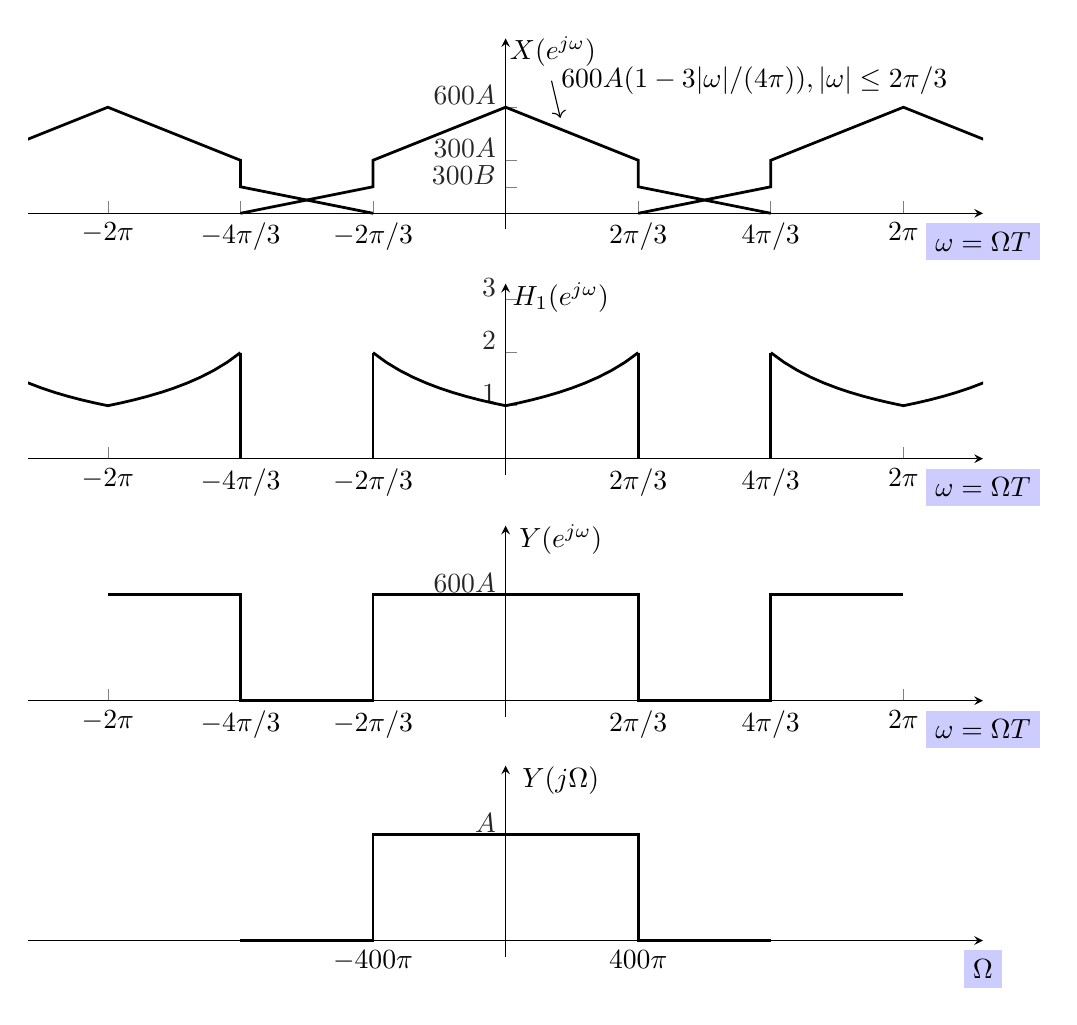
\begin{tikzpicture}
\begin{axis}[
	name=plot1,
	%at=(plot2.below south east), anchor=above north east,
	axis lines*=middle,
	enlargelimits = true,
	clip=true,
	scale only axis,
	width=\textwidth,
	height=0.2\textwidth,
	ymin=0, ymax=3,
	xmin=-8, xmax=8,
	axis line style={->,>=stealth},
	xlabel={\tikz[baseline]{\node[fill=blue!20,anchor=base] (t1) {$\omega = \Omega T$};}},
	ylabel={$X(e^{j\omega})$},
	every axis x label/.style={
		at={(ticklabel* cs:1)},
		%xshift=0.2cm,
		anchor=north,
	},
	every axis y label/.style={
		at={(ticklabel* cs:0.8)},
		anchor=south,
		xshift=0.6cm,
	},
	ytick={0.5, 1, 2},
	yticklabels={$300B$, $300A$, $600A$},
	yticklabel style={yshift=0.15cm},
	xtick={-8, -5.33, -2.666, 2.666, 5.33, 8},
	xticklabels={$-2\pi$, $-4\pi/3$, $-2\pi/3$, $2\pi/3$, $4\pi/3$, $2\pi$}, 
	every outer y axis line/.append style={white!15!black},
	every y tick label/.append style={font=\color{white!15!black}},
	legend style={draw=white!15!black,fill=white,legend cell align=left}]
	\addplot[solid, line width=1pt] coordinates {(-16/3, 0) (-8/3, 1/2) (-8/3, 1) (0, 2) (8/3, 1) (8/3, 1/2) (16/3, 0)};
	\addplot[solid, line width=1pt] coordinates {(-16/3-8, 0) (-8/3-8, 1/2) (-8/3-8, 1) (0-8, 2) (8/3-8, 1) (8/3-8, 1/2) (16/3-8, 0)};
	\addplot[solid, line width=1pt] coordinates {(-16/3+8, 0) (-8/3+8, 1/2) (-8/3+8, 1) (0+8, 2) (8/3+8, 1) (8/3+8, 1/2) (16/3+8, 0)};
	\node (t1) at (axis cs: 5, 2.5) {$600A(1-3|\omega|/(4\pi)), |\omega|\leq2\pi/3$};
	\draw[->] (t1.west) to (axis cs: 1.1, 1.8) {};
\end{axis}

\begin{axis}[
	name=plot2,
	at=(plot1.below south east), anchor=above north east,
	axis lines*=middle,
	enlargelimits = true,
	clip=true,
	scale only axis,
	width=\textwidth,
	height=0.2\textwidth,
	ymin=0, ymax=3,
	xmin=-8, xmax=8,
	axis line style={->,>=stealth},
	xlabel={\tikz[baseline]{\node[fill=blue!20,anchor=base] (t1) {$\omega = \Omega T$};}},
	ylabel={$H_1(e^{j\omega})$},
	every axis x label/.style={
		at={(ticklabel* cs:1)},
		%xshift=0.2cm,
		anchor=north,
	},
	every axis y label/.style={
		at={(ticklabel* cs:0.8)},
		anchor=south,
		xshift=0.7cm,
	},
	yticklabel style={yshift=0.15cm},
	xtick={-8, -5.33, -2.666, 2.666, 5.33, 8},
	xticklabels={$-2\pi$, $-4\pi/3$, $-2\pi/3$, $2\pi/3$, $4\pi/3$, $2\pi$}, 
	every outer y axis line/.append style={white!15!black},
	every y tick label/.append style={font=\color{white!15!black}},
	legend style={draw=white!15!black,fill=white,legend cell align=left}]
	\addplot[solid, line width=1pt, domain=-2.6667:2.6667, samples=21] {(1/(1-3*abs(x*pi/4)/(4*pi)))};
	\addplot[solid, line width=1pt, domain=-2.6667:2.6667, samples=21] ({x-8}, { 1/(1-3*abs(x*pi/4)/(4*pi))});
	\addplot[solid, line width=1pt, domain=-2.6667:2.6667, samples=21] ({x+8}, { 1/(1-3*abs(x*pi/4)/(4*pi))});
	\addplot[solid, line width=1pt] coordinates {(-2.6667, 2) (-2.6667, 0)};
	\addplot[solid, line width=1pt] coordinates {(2.6667, 2) (2.6667, 0)};
	\addplot[solid, line width=1pt] coordinates {(-2.6667+8, 2) (-2.6667+8, 0)};
	\addplot[solid, line width=1pt] coordinates {(2.6667-8, 2) (2.6667-8, 0)};
\end{axis}

\begin{axis}[
name=plot3,
at=(plot2.below south east), anchor=above north east,
axis lines*=middle,
enlargelimits = true,
clip=true,
scale only axis,
width=\textwidth,
height=0.2\textwidth,
ymin=0, ymax=3,
xmin=-8, xmax=8,
axis line style={->,>=stealth},
xlabel={\tikz[baseline]{\node[fill=blue!20,anchor=base] (t1) {$\omega = \Omega T$};}},
ylabel={$Y(e^{j\omega})$},
every axis x label/.style={
	at={(ticklabel* cs:1)},
	%xshift=0.2cm,
	anchor=north,
},
every axis y label/.style={
	at={(ticklabel* cs:0.8)},
	anchor=south,
	xshift=0.7cm,
},
yticklabel style={yshift=0.15cm},
ytick=2,
yticklabels=$600A$,
xtick={-8, -5.33, -2.666, 2.666, 5.33, 8},
xticklabels={$-2\pi$, $-4\pi/3$, $-2\pi/3$, $2\pi/3$, $4\pi/3$, $2\pi$}, 
every outer y axis line/.append style={white!15!black},
every y tick label/.append style={font=\color{white!15!black}},
legend style={draw=white!15!black,fill=white,legend cell align=left}]
\addplot[solid, line width=1pt] coordinates {(-8, 2) (2.6667-8, 2) (2.6667-8, 0) (-2.6667, 0) (-2.6667, 2) (2.6667, 2) (2.6667, 0) (-2.6667+8, 0) (-2.6667+8, 2) (8, 2)};
\end{axis}

\begin{axis}[
name=plot4,
at=(plot3.below south east), anchor=above north east,
axis lines*=middle,
enlargelimits = true,
clip=true,
scale only axis,
width=\textwidth,
height=0.2\textwidth,
ymin=0, ymax=3,
xmin=-8, xmax=8,
axis line style={->,>=stealth},
xlabel={\tikz[baseline]{\node[fill=blue!20,anchor=base] (t1) {$\Omega$};}},
ylabel={$Y(j\Omega)$},
every axis x label/.style={
	at={(ticklabel* cs:1)},
	%xshift=0.2cm,
	anchor=north,
},
every axis y label/.style={
	at={(ticklabel* cs:0.8)},
	anchor=south,
	xshift=0.7cm,
},
yticklabel style={yshift=0.15cm},
ytick=2,
yticklabels=$A$,
xtick={-2.666, 2.666},
xticklabels={$-400\pi$, $400\pi$}, 
every outer y axis line/.append style={white!15!black},
every y tick label/.append style={font=\color{white!15!black}},
legend style={draw=white!15!black,fill=white,legend cell align=left}]
\addplot[solid, line width=1pt] coordinates {(2.6667-8, 0) (-2.6667, 0) (-2.6667, 2) (2.6667, 2) (2.6667, 0) (-2.6667+8, 0)};
\end{axis}
\end{tikzpicture}}

The filter $H_1(e^{j\omega})$ only needs to flatten the frequency response of $X(e^{j\omega})$ over the interval $\omega < 2\pi/3$. Therefore,
\begin{equation}
H_1(e^{j\omega}) = \begin{cases}
\frac{1}{1 - \displaystyle\frac{3|\omega|}{4\pi}}, & |\omega|\leq \frac{2\pi}{3} \\
0, & \frac{2\pi}{3} < |\omega|\leq \pi
\end{cases}
\end{equation}
		
\subsection{(d)}

\resizebox{\linewidth}{!}{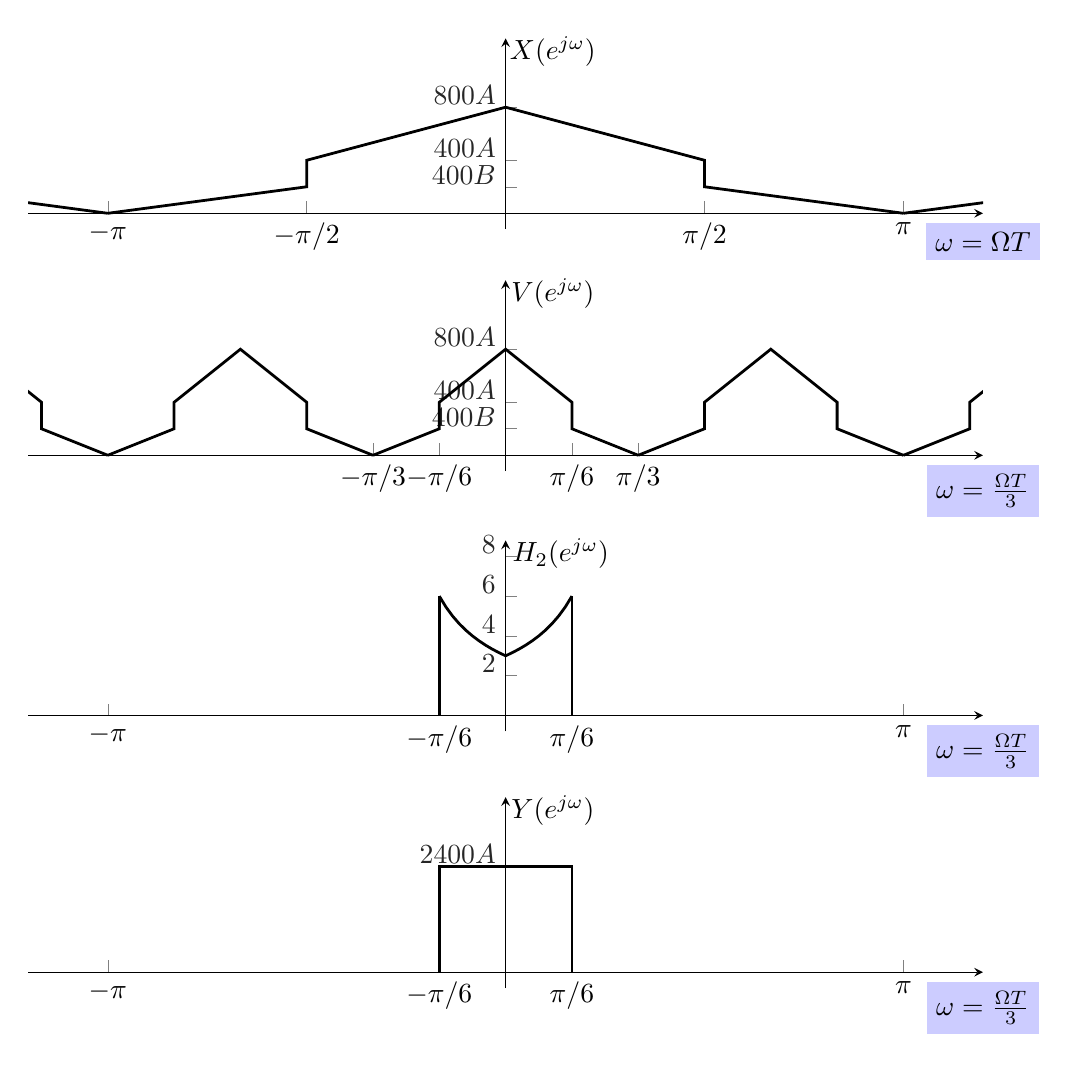
\begin{tikzpicture}
\begin{axis}[
name=plot1,
%at=(plot2.below south east), anchor=above north east,
axis lines*=middle,
enlargelimits = true,
clip=true,
scale only axis,
width=\textwidth,
height=0.2\textwidth,
ymin=0, ymax=3,
xmin=-8, xmax=8,
axis line style={->,>=stealth},
xlabel={\tikz[baseline]{\node[fill=blue!20,anchor=base] (t1) {$\omega = \Omega T$};}},
ylabel={$X(e^{j\omega})$},
every axis x label/.style={
	at={(ticklabel* cs:1)},
	%xshift=0.2cm,
	anchor=north,
},
every axis y label/.style={
	at={(ticklabel* cs:0.8)},
	anchor=south,
	xshift=0.6cm,
},
ytick={0.5, 1, 2},
yticklabels={$400B$, $400A$, $800A$},
yticklabel style={yshift=0.15cm},
xtick={-8, -4, 4, 8},
xticklabels={$-\pi$, $-\pi/2$, $\pi/2$, $\pi$}, 
every outer y axis line/.append style={white!15!black},
every y tick label/.append style={font=\color{white!15!black}},
legend style={draw=white!15!black,fill=white,legend cell align=left}]
\def\fs{16}
\foreach \k in {-1, 0, 1}{
	\addplot[solid, line width=1pt] coordinates {(-8+\k*\fs, 0) (-4+\k*\fs, 1/2) (-4+\k*\fs, 1) (0+\k*\fs, 2) (4+\k*\fs, 1) (4+\k*\fs, 1/2) (8+\k*\fs, 0)};	
}
\end{axis}

\begin{axis}[
name=plot2,
at=(plot1.below south east), anchor=above north east,
axis lines*=middle,
enlargelimits = true,
clip=true,
scale only axis,
width=\textwidth,
height=0.2\textwidth,
ymin=0, ymax=3,
xmin=-24, xmax=24,
axis line style={->,>=stealth},
xlabel={\tikz[baseline]{\node[fill=blue!20,anchor=base] (t1) {$\omega = \frac{\Omega T}{3}$};}},
ylabel={$V(e^{j\omega})$},
every axis x label/.style={
	at={(ticklabel* cs:1)},
	%xshift=0.2cm,
	anchor=north,
},
every axis y label/.style={
	at={(ticklabel* cs:0.8)},
	anchor=south,
	xshift=0.6cm,
},
ytick={0.5, 1, 2},
yticklabels={$400B$, $400A$, $800A$},
yticklabel style={yshift=0.15cm},
xtick={-8, -4, 4, 8},
xticklabels={$-\pi/3$, $-\pi/6$, $\pi/6$, $\pi/3$}, 
every outer y axis line/.append style={white!15!black},
every y tick label/.append style={font=\color{white!15!black}},
legend style={draw=white!15!black,fill=white,legend cell align=left}]
\def\fs{16}
\foreach \k in {-2, -1, 0, 1, 2}{
	\addplot[solid, line width=1pt] coordinates {(-8+\k*\fs, 0) (-4+\k*\fs, 1/2) (-4+\k*\fs, 1) (0+\k*\fs, 2) (4+\k*\fs, 1) (4+\k*\fs, 1/2) (8+\k*\fs, 0)};	
}

\end{axis}

\begin{axis}[
name=plot3,
at=(plot2.below south east), anchor=above north east,
axis lines*=middle,
enlargelimits = true,
clip=true,
scale only axis,
width=\textwidth,
height=0.2\textwidth,
ymin=0, ymax=8,
xmin=-24, xmax=24,
axis line style={->,>=stealth},
xlabel={\tikz[baseline]{\node[fill=blue!20,anchor=base] (t1) {$\omega = \frac{\Omega T}{3}$};}},
ylabel={$H_2(e^{j\omega})$},
every axis x label/.style={
	at={(ticklabel* cs:1)},
	%xshift=0.2cm,
	anchor=north,
},
every axis y label/.style={
	at={(ticklabel* cs:0.8)},
	anchor=south,
	xshift=0.7cm,
},
yticklabel style={yshift=0.15cm},
xtick={-24, -4, 4, 24},
xticklabels={$-\pi$, $-\pi/6$, $\pi/6$, $\pi$}, 
every outer y axis line/.append style={white!15!black},
every y tick label/.append style={font=\color{white!15!black}},
legend style={draw=white!15!black,fill=white,legend cell align=left}]
\addplot[solid, line width=1pt, domain=-4:4, samples=21] {3/(1-3*abs(x/4*pi/6)/pi)};
\addplot[solid, line width=1pt] coordinates {(-4, 0) (-4, 6)};
\addplot[solid, line width=1pt] coordinates {(4, 0) (4, 6)};
\end{axis}

\begin{axis}[
name=plot4,
at=(plot3.below south east), anchor=above north east,
axis lines*=middle,
enlargelimits = true,
clip=true,
scale only axis,
width=\textwidth,
height=0.2\textwidth,
ymin=0, ymax=3,
xmin=-24, xmax=24,
axis line style={->,>=stealth},
xlabel={\tikz[baseline]{\node[fill=blue!20,anchor=base] (t1) {$\omega = \frac{\Omega T}{3}$};}},
ylabel={$Y(e^{j\omega})$},
every axis x label/.style={
	at={(ticklabel* cs:1)},
	%xshift=0.2cm,
	anchor=north,
},
every axis y label/.style={
	at={(ticklabel* cs:0.8)},
	anchor=south,
	xshift=0.6cm,
},
ytick={2},
yticklabels={$2400A$},
yticklabel style={yshift=0.15cm},
xtick={-24, -4, 4, 24},
xticklabels={$-\pi$, $-\pi/6$, $\pi/6$, $\pi$}, 
every outer y axis line/.append style={white!15!black},
every y tick label/.append style={font=\color{white!15!black}},
legend style={draw=white!15!black,fill=white,legend cell align=left}]
\addplot[solid, line width=1pt] coordinates {(-4, 0) (-4, 2) (4, 2) (4, 0)};
\end{axis}

\end{tikzpicture}
}

The filter $H_2(e^{j\omega})$ only needs to flatten the frequency response of $V(e^{j\omega})$ over the interval $\omega < \pi/6$. Therefore,
\begin{equation}
H_2(e^{j\omega}) = \begin{cases}
\frac{3}{1 - \displaystyle\frac{3|\omega|}{\pi}}, & |\omega|\leq \frac{\pi}{6} \\
0, & \frac{\pi}{6} < |\omega|\leq \pi
\end{cases}
\end{equation}

\section{Problem 2}
\subsection{(a)}

To maintain a constant time scale we need
\begin{equation}
T_2 = \frac{2}{3}T_1
\end{equation}

\subsection{(b)}

To avoid aliasing in the sampling of the input
\begin{align}
\Omega_s &= \frac{2\pi}{T_1} > 2\Omega_N = 8000\pi \\
T_1 &< 1/4000
\end{align}

To perfectly reconstruct the input, we should preserve the same time scale between input and output. Hence, using the result from part (a):

\begin{equation}
T_2 = \frac{2}{3}T_1 \implies T_2 > 1/6000
\end{equation}

\subsection{(c)}
\begin{center}
	\resizebox{0.8\linewidth}{!}{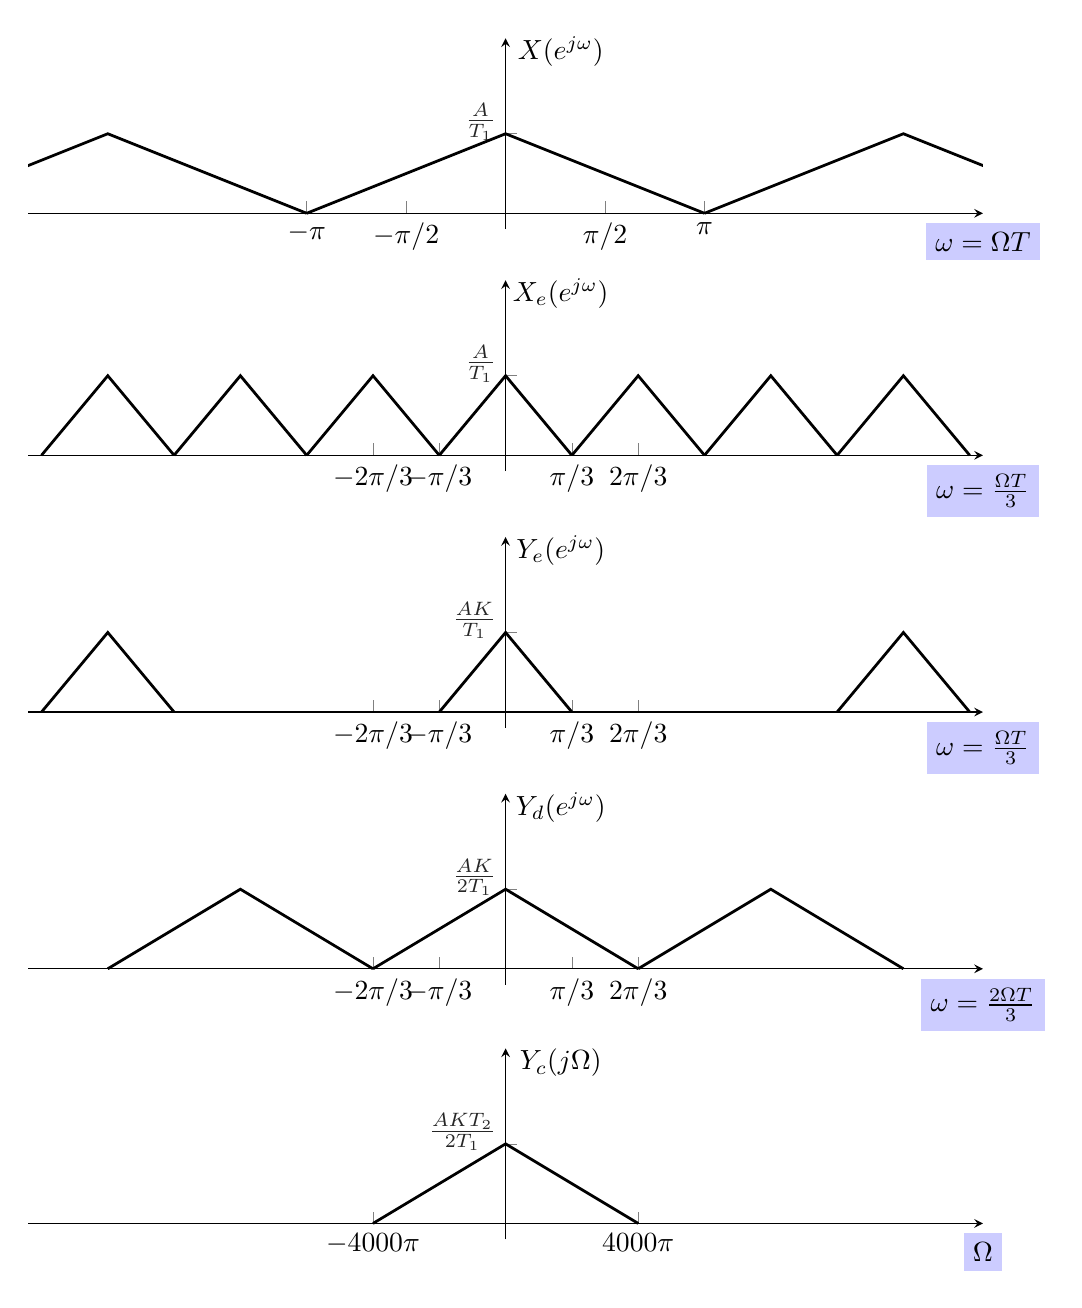
\begin{tikzpicture}
\begin{axis}[
name=plot1,
%at=(plot2.below south east), anchor=above north east,
axis lines*=middle,
enlargelimits = true,
clip=true,
scale only axis,
width=\textwidth,
height=0.2\textwidth,
ymin=0, ymax=2,
xmin=-16, xmax=16,
axis line style={->,>=stealth},
xlabel={\tikz[baseline]{\node[fill=blue!20,anchor=base] (t1) {$\omega=\Omega T$};}},
ylabel={$X(e^{j\omega})$},
every axis x label/.style={
	at={(ticklabel* cs:1)},
	%xshift=0.2cm,
	anchor=north,
},
every axis y label/.style={
	at={(ticklabel* cs:0.8)},
	anchor=south,
	xshift=0.7cm,
},
ytick={1},
yticklabels={$\frac{A}{T_1}$},
yticklabel style={yshift=0.15cm},
xtick={-8, -4, 4, 8},
xticklabels={$-\pi$, $-\pi/2$, $\pi/2$, $\pi$}, 
every outer y axis line/.append style={white!15!black},
every y tick label/.append style={font=\color{white!15!black}},
legend style={draw=white!15!black,fill=white,legend cell align=left}]
\def\fs{16}
\foreach \k in {-1, 0, 1}{
	\addplot[solid, line width=1pt] coordinates {(-8+\k*\fs, 0) (0+\k*\fs, 1) (8+\k*\fs, 0)};	
}
\end{axis}

\begin{axis}[
name=plot2,
at=(plot1.below south east), anchor=above north east,
axis lines*=middle,
enlargelimits = true,
clip=true,
scale only axis,
width=\textwidth,
height=0.2\textwidth,
ymin=0, ymax=2,
xmin=-16, xmax=16,
axis line style={->,>=stealth},
xlabel={\tikz[baseline]{\node[fill=blue!20,anchor=base] (t1) {$\omega = \frac{\Omega T}{3}$};}},
ylabel={$X_e(e^{j\omega})$},
every axis x label/.style={
	at={(ticklabel* cs:1)},
	%xshift=0.2cm,
	anchor=north,
},
every axis y label/.style={
	at={(ticklabel* cs:0.8)},
	anchor=south,
	xshift=0.7cm,
},
ytick={1},
yticklabels={$\frac{A}{T_1}$},
yticklabel style={yshift=0.15cm},
xtick={-5.3333, -2.6667, 2.6667, 5.3333},
xticklabels={$-2\pi/3$, $-\pi/3$, $\pi/3$, $2\pi/3$},
every outer y axis line/.append style={white!15!black},
every y tick label/.append style={font=\color{white!15!black}},
legend style={draw=white!15!black,fill=white,legend cell align=left}]
\def\fs{5.3333}
\foreach \k in {-3, -2, -1, 0, 1, 2, 3}{
	\addplot[solid, line width=1pt] coordinates {(-8/3+\k*\fs, 0) (0+\k*\fs, 1) (8/3+\k*\fs, 0)};	
}
\end{axis}

\begin{axis}[
name=plot3,
at=(plot2.below south east), anchor=above north east,
axis lines*=middle,
enlargelimits = true,
clip=true,
scale only axis,
width=\textwidth,
height=0.2\textwidth,
ymin=0, ymax=2,
xmin=-16, xmax=16,
axis line style={->,>=stealth},
xlabel={\tikz[baseline]{\node[fill=blue!20,anchor=base] (t1) {$\omega = \frac{\Omega T}{3}$};}},
ylabel={$Y_e(e^{j\omega})$},
every axis x label/.style={
	at={(ticklabel* cs:1)},
	%xshift=0.2cm,
	anchor=north,
},
every axis y label/.style={
	at={(ticklabel* cs:0.8)},
	anchor=south,
	xshift=0.7cm,
},
ytick={1},
yticklabels={$\frac{AK}{T_1}$},
yticklabel style={yshift=0.15cm},
xtick={-5.3333, -2.6667, 2.6667, 5.3333},
xticklabels={$-2\pi/3$, $-\pi/3$, $\pi/3$, $2\pi/3$},
every outer y axis line/.append style={white!15!black},
every y tick label/.append style={font=\color{white!15!black}},
legend style={draw=white!15!black,fill=white,legend cell align=left}]
\def\fs{5.3333}
\foreach \k in {-3, 0,  3}{
	\addplot[solid, line width=1pt] coordinates {(-8/3+\k*\fs, 0) (0+\k*\fs, 1) (8/3+\k*\fs, 0)};	
}
\end{axis}

\begin{axis}[
name=plot4,
at=(plot3.below south east), anchor=above north east,
axis lines*=middle,
enlargelimits = true,
clip=true,
scale only axis,
width=\textwidth,
height=0.2\textwidth,
ymin=0, ymax=2,
xmin=-16, xmax=16,
axis line style={->,>=stealth},
xlabel={\tikz[baseline]{\node[fill=blue!20,anchor=base] (t1) {$\omega = \frac{2\Omega T}{3}$};}},
ylabel={$Y_d(e^{j\omega})$},
every axis x label/.style={
	at={(ticklabel* cs:1)},
	%xshift=0.2cm,
	anchor=north,
},
every axis y label/.style={
	at={(ticklabel* cs:0.8)},
	anchor=south,
	xshift=0.7cm,
},
ytick={1},
yticklabels={$\frac{AK}{2T_1}$},
yticklabel style={yshift=0.15cm},
xtick={-5.3333, -2.6667, 2.6667, 5.3333},
xticklabels={$-2\pi/3$, $-\pi/3$, $\pi/3$, $2\pi/3$},
every outer y axis line/.append style={white!15!black},
every y tick label/.append style={font=\color{white!15!black}},
legend style={draw=white!15!black,fill=white,legend cell align=left}]
\def\fs{10.6667}
\foreach \k in {-1, 0, 1}{
	\addplot[solid, line width=1pt] coordinates {(-16/3+\k*\fs, 0) (0+\k*\fs, 1) (16/3+\k*\fs, 0)};	
}
\end{axis}


\begin{axis}[
name=plot5,
at=(plot4.below south east), anchor=above north east,
axis lines*=middle,
enlargelimits = true,
clip=true,
scale only axis,
width=\textwidth,
height=0.2\textwidth,
ymin=0, ymax=2,
xmin=-16, xmax=16,
axis line style={->,>=stealth},
xlabel={\tikz[baseline]{\node[fill=blue!20,anchor=base] (t1) {$\Omega$};}},
ylabel={$Y_c(j\Omega)$},
every axis x label/.style={
	at={(ticklabel* cs:1)},
	%xshift=0.2cm,
	anchor=north,
},
every axis y label/.style={
	at={(ticklabel* cs:0.8)},
	anchor=south,
	xshift=0.7cm,
},
ytick={1},
yticklabels={$\frac{AKT_2}{2T_1}$},
yticklabel style={yshift=0.15cm},
xtick={-5.3333, 5.3333},
xticklabels={$-4000\pi$, $4000\pi$},
every outer y axis line/.append style={white!15!black},
every y tick label/.append style={font=\color{white!15!black}},
legend style={draw=white!15!black,fill=white,legend cell align=left}]
\def\fs{10.6667}
\foreach \k in {0}{
	\addplot[solid, line width=1pt] coordinates {(-16/3+\k*\fs, 0) (0+\k*\fs, 1) (16/3+\k*\fs, 0)};	
}
\end{axis}
\end{tikzpicture}
}
\end{center}

For perfect reconstruction we need: 
\begin{equation}
\frac{AKT_2}{2T} = A \implies K = \frac{2T_1}{T_2} = 3
\end{equation}

Therefore,

\begin{equation}
H(e^{j\omega}) = \begin{cases}
3, &|\omega|\leq \pi/3 \\
0, &\pi/3 < |\omega| \leq \pi
\end{cases}
\end{equation}

\subsection{(d)}

\begin{equation}
y_c(t) = 2x_c(t-4T_1) \Longleftrightarrow Y_c(j\Omega) = 2e^{-j4T_1\Omega}X_c(j\Omega)
\end{equation}

Similarly to previous items, the shape of the spectrum will not be changed, so we can focus on the amplitude at $\Omega = 0$ in order to determine the amplitude of $H(e^{j\omega})$. 

\begin{align*}
Y_c(j\Omega = 0) &= 2Ae^{-j4T_1\Omega} \\
Y_d(e^{j\omega} = 1) &= \frac{2A}{T_2}e^{-j4T_1\omega/T_2} = \frac{2A}{T_2}e^{-j6\omega} \tag{since we can interpret $y_d[n] = y_c(nT_2)$} \\
Y_e(e^{j\omega} = 1) &= \frac{4A}{T_2}e^{-j16\omega} \tag{upsampling by 2 with filter scaling 2} \\
\end{align*}

By comparing $Y_e(e^{j\omega} = 1)$ and $X_e(j\Omega)$, we can write

\begin{align} \nonumber
H(e^{j\omega}) &= \begin{cases}
4\frac{T_1}{T_2}e^{-j12\omega}, & |\omega|\leq \pi/3 \\
0, &\pi/3 < |\omega| \leq \pi
\end{cases} \\
&= \begin{cases}
6e^{-j12\omega}, & |\omega|\leq \pi/3 \\
0, &\pi/3 < |\omega| \leq \pi
\end{cases}
\end{align}

\subsection{(e)}

\begin{center}
	\resizebox{\linewidth}{!}{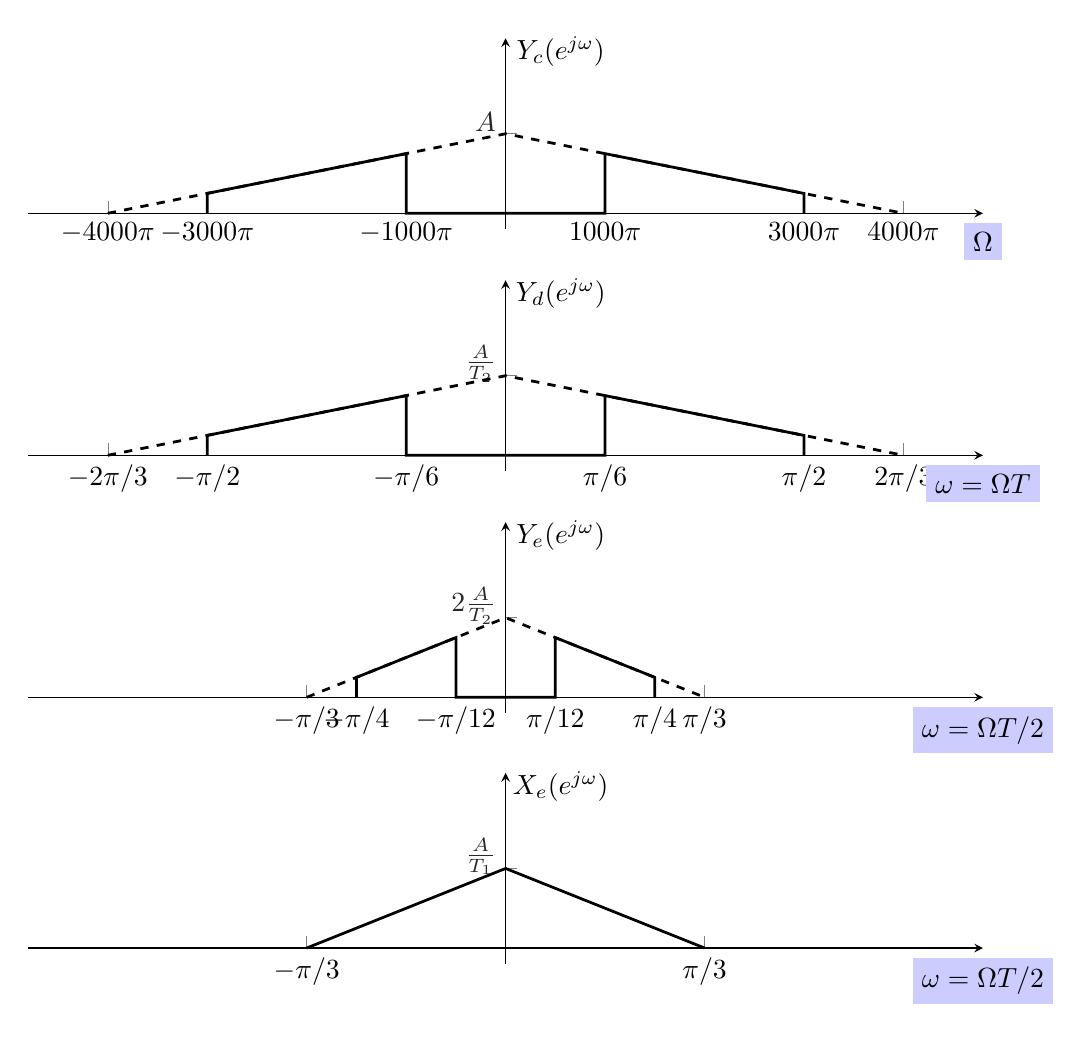
\begin{tikzpicture}
\begin{axis}[
name=plot1,
%at=(plot2.below south east), anchor=above north east,
axis lines*=middle,
enlargelimits = true,
clip=true,
scale only axis,
width=\textwidth,
height=0.2\textwidth,
ymin=0, ymax=2,
xmin=-8, xmax=8,
axis line style={->,>=stealth},
xlabel={\tikz[baseline]{\node[fill=blue!20,anchor=base] (t1) {$\Omega$};}},
ylabel={$Y_c(e^{j\omega})$},
every axis x label/.style={
	at={(ticklabel* cs:1)},
	%xshift=0.2cm,
	anchor=north,
},
every axis y label/.style={
	at={(ticklabel* cs:0.8)},
	anchor=south,
	xshift=0.7cm,
},
ytick={1},
yticklabels={$A$},
yticklabel style={yshift=0.15cm},
xtick={-8, -6, -2, 2, 6, 8},
xticklabels={$-4000\pi$, $-3000\pi$, $-1000\pi$, $1000\pi$, $3000\pi$, $4000\pi$}, 
every outer y axis line/.append style={white!15!black},
every y tick label/.append style={font=\color{white!15!black}},
legend style={draw=white!15!black,fill=white,legend cell align=left}]
\addplot[dashed, line width=1pt] coordinates {(-8, 0) (0, 1) (8, 0)};	
\addplot[solid, line width=1pt] coordinates {(-6, 0) (-6, 1/4) (-2, 3/4) (-2, 0) (2, 0) (2, 3/4) (6, 1/4) (6, 0)};	
\end{axis}

\begin{axis}[
name=plot2,
at=(plot1.below south east), anchor=above north east,
axis lines*=middle,
enlargelimits = true,
clip=true,
scale only axis,
width=\textwidth,
height=0.2\textwidth,
ymin=0, ymax=2,
xmin=-8, xmax=8,
axis line style={->,>=stealth},
xlabel={\tikz[baseline]{\node[fill=blue!20,anchor=base] (t1) {$\omega =\Omega T$};}},
ylabel={$Y_d(e^{j\omega})$},
every axis x label/.style={
	at={(ticklabel* cs:1)},
	%xshift=0.2cm,
	anchor=north,
},
every axis y label/.style={
	at={(ticklabel* cs:0.8)},
	anchor=south,
	xshift=0.7cm,
},
ytick={1},
yticklabels={$\frac{A}{T_2}$},
yticklabel style={yshift=0.15cm},
xtick={-8, -6, -2, 2, 6, 8},
xticklabels={$-2\pi/3$, $-\pi/2$, $-\pi/6$, $\pi/6$, $\pi/2$, $2\pi/3$}, 
every outer y axis line/.append style={white!15!black},
every y tick label/.append style={font=\color{white!15!black}},
legend style={draw=white!15!black,fill=white,legend cell align=left}]
\addplot[dashed, line width=1pt] coordinates {(-8, 0) (0, 1) (8, 0)};	
\addplot[solid, line width=1pt] coordinates {(-6, 0) (-6, 1/4) (-2, 3/4) (-2, 0) (2, 0) (2, 3/4) (6, 1/4) (6, 0)};	
\end{axis}

\begin{axis}[
name=plot3,
at=(plot2.below south east), anchor=above north east,
axis lines*=middle,
enlargelimits = true,
clip=true,
scale only axis,
width=\textwidth,
height=0.2\textwidth,
ymin=0, ymax=2,
xmin=-16, xmax=16,
axis line style={->,>=stealth},
xlabel={\tikz[baseline]{\node[fill=blue!20,anchor=base] (t1) {$\omega =\Omega T/2$};}},
ylabel={$Y_e(e^{j\omega})$},
every axis x label/.style={
	at={(ticklabel* cs:1)},
	%xshift=0.2cm,
	anchor=north,
},
every axis y label/.style={
	at={(ticklabel* cs:0.8)},
	anchor=south,
	xshift=0.7cm,
},
ytick={1},
yticklabels={$2\frac{A}{T_2}$},
yticklabel style={yshift=0.15cm},
xtick={-8, -6, -2, 2, 6, 8},
xticklabels={$-\pi/3$, $-\pi/4$, $-\pi/12$, $\pi/12$, $\pi/4$, $\pi/3$}, 
every outer y axis line/.append style={white!15!black},
every y tick label/.append style={font=\color{white!15!black}},
legend style={draw=white!15!black,fill=white,legend cell align=left}]
\addplot[dashed, line width=1pt] coordinates {(-8, 0) (0, 1) (8, 0)};	
\addplot[solid, line width=1pt] coordinates {(-6, 0) (-6, 1/4) (-2, 3/4) (-2, 0) (2, 0) (2, 3/4) (6, 1/4) (6, 0)};	
\end{axis}

\begin{axis}[
name=plot4,
at=(plot3.below south east), anchor=above north east,
axis lines*=middle,
enlargelimits = true,
clip=true,
scale only axis,
width=\textwidth,
height=0.2\textwidth,
ymin=0, ymax=2,
xmin=-16, xmax=16,
axis line style={->,>=stealth},
xlabel={\tikz[baseline]{\node[fill=blue!20,anchor=base] (t1) {$\omega =\Omega T/2$};}},
ylabel={$X_e(e^{j\omega})$},
every axis x label/.style={
	at={(ticklabel* cs:1)},
	%xshift=0.2cm,
	anchor=north,
},
every axis y label/.style={
	at={(ticklabel* cs:0.8)},
	anchor=south,
	xshift=0.7cm,
},
ytick={1},
yticklabels={$\frac{A}{T_1}$},
yticklabel style={yshift=0.15cm},
xtick={-8, 8},
xticklabels={$-\pi/3$, $\pi/3$}, 
every outer y axis line/.append style={white!15!black},
every y tick label/.append style={font=\color{white!15!black}},
legend style={draw=white!15!black,fill=white,legend cell align=left}]
\addplot[solid, line width=1pt] coordinates {(-8, 0) (0, 1) (8, 0)};	
%\addplot[solid, line width=1pt] coordinates {(-6, 0) (-6, 1/4) (-2, 3/4) (-2, 0) (2, 0) (2, 3/4) (6, 1/4) (6, 0)};	
\end{axis}

\end{tikzpicture}
}
\end{center}

Therefore, to obtain $Y_e(e^{j\omega})$ from $X(e^{j\omega})$, the filter $H(e^{j\omega})$ must satisfy
\begin{align} \nonumber
H(e^{j\omega}) &= \begin{cases}
0, & |\omega| \leq \pi/12\\
\frac{2T_1}{T_2}, & \pi/12 < |\omega| \leq \pi/4\\
0, & \pi/4 < |\omega| \leq \pi
\end{cases} \\
&= \begin{cases}
0, & |\omega| \leq \pi/12\\
3, & \pi/12 < |\omega| \leq \pi/4\\
0, & \pi/4 < |\omega| \leq \pi
\end{cases},
\end{align}
which is a band-pass filter.

\subsection{(f)}
\begin{equation}
y_c(t) = \dfrac{d}{dt}x_c(t) \Longleftrightarrow Y_c(j\Omega) = j\Omega X_c(j\Omega)
\end{equation}

\begin{center}
	\resizebox{\linewidth}{!}{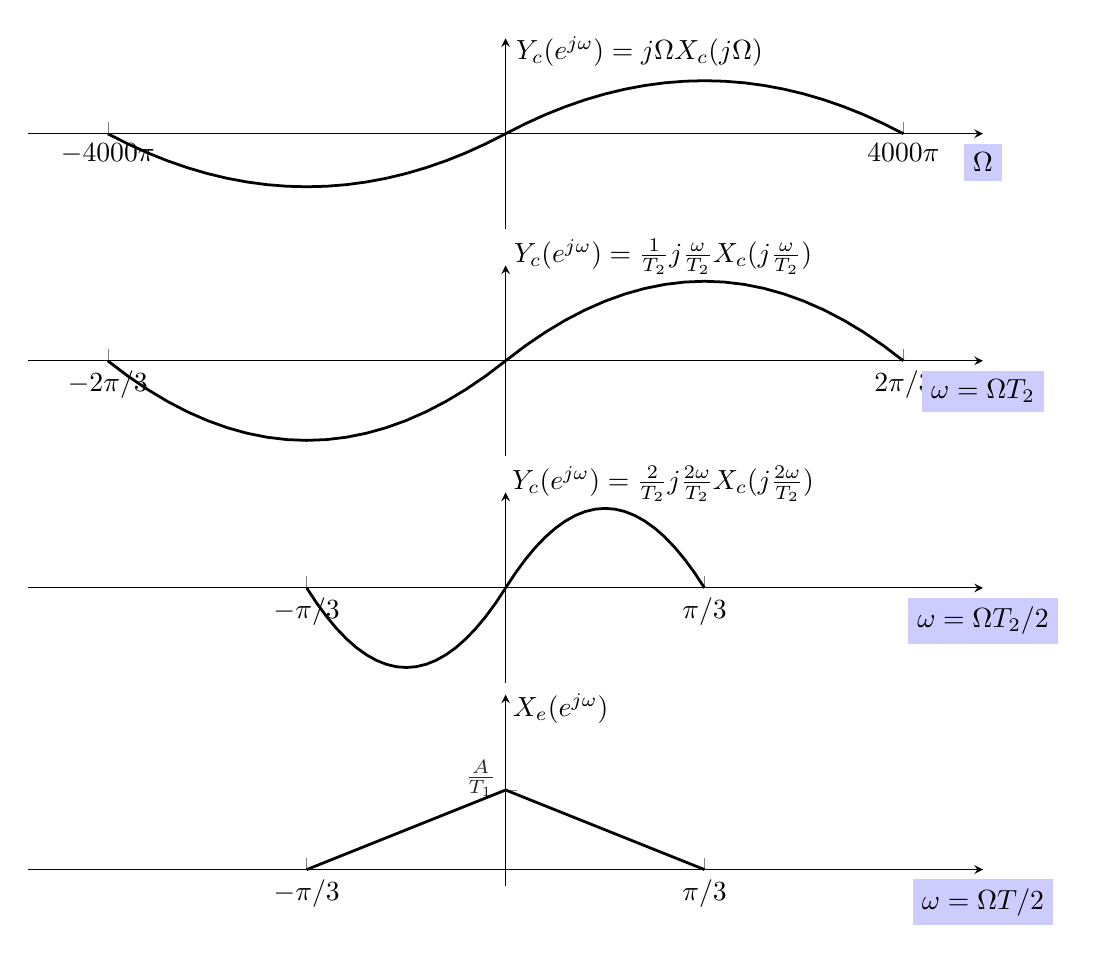
\begin{tikzpicture}
\begin{axis}[
name=plot1,
%at=(plot2.below south east), anchor=above north east,
axis lines*=middle,
enlargelimits = true,
clip=true,
scale only axis,
width=\textwidth,
height=0.2\textwidth,
ymin=-3, ymax=3,
xmin=-8, xmax=8,
axis line style={->,>=stealth},
xlabel={\tikz[baseline]{\node[fill=blue!20,anchor=base] (t1) {$\Omega$};}},
ylabel={$Y_c(e^{j\omega}) = j\Omega X_c(j\Omega)$},
every axis x label/.style={
	at={(ticklabel* cs:1)},
	%xshift=0.2cm,
	anchor=north,
},
every axis y label/.style={
	at={(ticklabel* cs:0.8)},
	anchor=south,
	xshift=1.7cm,
},
ytick=\empty,
yticklabels={$A$},
yticklabel style={yshift=0.15cm},
xtick={-8, 8},
xticklabels={$-4000\pi$, $4000\pi$}, 
every outer y axis line/.append style={white!15!black},
every y tick label/.append style={font=\color{white!15!black}},
legend style={draw=white!15!black,fill=white,legend cell align=left}]
\addplot[solid, line width=1pt, domain=-8:0, samples=21] {x*(1/8*x+1)};	
\addplot[solid, line width=1pt, domain=0:8, samples=21] {x*(-1/8*x+1)};
\end{axis}

\begin{axis}[
name=plot2,
at=(plot1.below south east), anchor=above north east,
axis lines*=middle,
enlargelimits = true,
clip=true,
scale only axis,
width=\textwidth,
height=0.2\textwidth,
%ymin=-3, ymax=3,
xmin=-8, xmax=8,
axis line style={->,>=stealth},
xlabel={\tikz[baseline]{\node[fill=blue!20,anchor=base] (t1) {$\omega = \Omega T_2$};}},
ylabel={$Y_c(e^{j\omega})  = \frac{1}{T_2}j\frac{\omega}{T_2} X_c(j\frac{\omega}{T_2})$},
every axis x label/.style={
	at={(ticklabel* cs:1)},
	%xshift=0.2cm,
	anchor=north,
},
every axis y label/.style={
	at={(ticklabel* cs:0.9)},
	anchor=south,
	xshift=2cm,
},
ytick=\empty,
yticklabels={$A$},
yticklabel style={yshift=0.15cm},
xtick={-8, 8},
xticklabels={$-2\pi/3$, $2\pi/3$}, 
every outer y axis line/.append style={white!15!black},
every y tick label/.append style={font=\color{white!15!black}},
legend style={draw=white!15!black,fill=white,legend cell align=left}]
\addplot[solid, line width=1pt, domain=-8:0, samples=21] {x*(1/8*x+1)};	
\addplot[solid, line width=1pt, domain=0:8, samples=21] {x*(-1/8*x+1)};
\end{axis}

\begin{axis}[
name=plot3,
at=(plot2.below south east), anchor=above north east,
axis lines*=middle,
enlargelimits = true,
clip=true,
scale only axis,
width=\textwidth,
height=0.2\textwidth,
%ymin=-3, ymax=3,
xmin=-16, xmax=16,
axis line style={->,>=stealth},
xlabel={\tikz[baseline]{\node[fill=blue!20,anchor=base] (t1) {$\omega = \Omega T_2/2$};}},
ylabel={$Y_c(e^{j\omega})= \frac{2}{T_2}j\frac{2\omega}{T_2} X_c(j\frac{2\omega}{T_2})$},
every axis x label/.style={
	at={(ticklabel* cs:1)},
	%xshift=0.2cm,
	anchor=north,
},
every axis y label/.style={
	at={(ticklabel* cs:0.9)},
	anchor=south,
	xshift=2cm,
},
ytick=\empty,
yticklabels={$A$},
yticklabel style={yshift=0.15cm},
xtick={-8,8},
xticklabels={$-\pi/3$, $\pi/3$}, 
every outer y axis line/.append style={white!15!black},
every y tick label/.append style={font=\color{white!15!black}},
legend style={draw=white!15!black,fill=white,legend cell align=left}]
\addplot[solid, line width=1pt, domain=-8:0, samples=21] {x*(1/8*x+1)};	
\addplot[solid, line width=1pt, domain=0:8, samples=21] {x*(-1/8*x+1)};
\end{axis}

\begin{axis}[
name=plot4,
at=(plot3.below south east), anchor=above north east,
axis lines*=middle,
enlargelimits = true,
clip=true,
scale only axis,
width=\textwidth,
height=0.2\textwidth,
ymin=0, ymax=2,
xmin=-16, xmax=16,
axis line style={->,>=stealth},
xlabel={\tikz[baseline]{\node[fill=blue!20,anchor=base] (t1) {$\omega =\Omega T/2$};}},
ylabel={$X_e(e^{j\omega})$},
every axis x label/.style={
	at={(ticklabel* cs:1)},
	%xshift=0.2cm,
	anchor=north,
},
every axis y label/.style={
	at={(ticklabel* cs:0.8)},
	anchor=south,
	xshift=0.7cm,
},
ytick={1},
yticklabels={$\frac{A}{T_1}$},
yticklabel style={yshift=0.15cm},
xtick={-8, 8},
xticklabels={$-\pi/3$, $\pi/3$}, 
every outer y axis line/.append style={white!15!black},
every y tick label/.append style={font=\color{white!15!black}},
legend style={draw=white!15!black,fill=white,legend cell align=left}]
\addplot[solid, line width=1pt] coordinates {(-8, 0) (0, 1) (8, 0)};	
%\addplot[solid, line width=1pt] coordinates {(-6, 0) (-6, 1/4) (-2, 3/4) (-2, 0) (2, 0) (2, 3/4) (6, 1/4) (6, 0)};	
\end{axis}

\end{tikzpicture}
}
\end{center}

Since for $|\omega|\leq \pi/3$, $X_c(j2\omega/T_2) = X_c(j3\omega/T_1) = T_1X_e(e^{j\omega})$. Thus,
\begin{align} \nonumber
Y_e(e^{j\omega}) &= 4j\frac{\omega}{T_2}X_c(j2\frac{\omega}{T_2}) \\ \nonumber
&= 4j\frac{\omega}{T_2^2}T_1X_e(e^{j\omega}) \\ 
&= 4j\frac{T_1}{T_2^2}\omega X_e(e^{j\omega}), |\omega|\leq\pi/3 
\end{align}

Therefore,

\begin{align}
H(e^{j\omega}) &= \begin{cases}
4j\frac{T_1}{T_2^2}\omega, & |\omega|\leq \pi/3 \\
0, &\pi/3 < |\omega| \leq \pi
\end{cases}
\end{align}

\section{Problem 3}

\subsection{(a)}
For the original system
\begin{align} \nonumber
\mathcal{F}\{\phi_1[m]\} &= |X_1(e^{j\omega})|^2 \\ \nonumber
&= |X_e(e^{j\omega L})H_1(e^{j\omega})|^2 \\ 
& = \begin{cases}
L^2|X_e(e^{j\omega L})|^2, & |\omega| \leq \pi/L \\
0, & \pi/L < |\omega| \leq \pi
\end{cases} 
\end{align}

For the system proposed by the student
\begin{align} \nonumber
\mathcal{F}\{\phi_3[m]\} &= \mathcal{F}\{\phi_{2e}[m]\} H_2(e^{j\omega}) \\
&= |X(e^{j\omega L})|^2H_2(e^{j\omega})
\end{align}

The two systems will be equivalent if
\begin{equation}
H_2(e^{j\omega}) = \begin{cases}
L^2, & |\omega| \leq \pi/L \\
0, & \pi/L < |\omega| \leq \pi
\end{cases}
\end{equation}

\subsection{(b)}

\begin{align} \nonumber
\mathcal{F}\{\phi_5[m]\} &= |X(e^{j\omega L})|^2 H_3(e^{j\omega})
\end{align}

This is exactly the same condition of part (a). Therefore, 

\begin{equation}
H_3(e^{j\omega}) = \begin{cases}
L^2, & |\omega| \leq \pi/L \\
0, & \pi/L < |\omega| \leq \pi
\end{cases}
\end{equation}

\section{Problem 4}

\noindent\textbf{Part 1: Implementing a quantizer}
\subsection{(a)}

The quantizer function implemented is shown below. Many other implementations are possible and will be accepted.

% This file was automatically created from the m-file 
% "m2tex.m" written by USL. 
% The fontencoding in this file is UTF-8. 
%  
% You will need to include the following two packages in 
% your LaTeX-Main-File. 
%  
% \usepackage{color} 
% \usepackage{fancyvrb} 
%  
% It is advised to use the following option for Inputenc 
% \usepackage[utf8]{inputenc} 
%  
  
% definition of matlab colors: 
\definecolor{mblue}{rgb}{0,0,1} 
\definecolor{mgreen}{rgb}{0.13333,0.5451,0.13333} 
\definecolor{mred}{rgb}{0.62745,0.12549,0.94118} 
\definecolor{mgrey}{rgb}{0.5,0.5,0.5} 
\definecolor{mdarkgrey}{rgb}{0.25,0.25,0.25} 
  
\DefineShortVerb[fontfamily=courier,fontseries=m]{\$} 
\DefineShortVerb[fontfamily=courier,fontseries=b]{\#} 
  
\noindent               
 \hspace*{-1.6em}{\scriptsize 1}$  $#function#$ [xq, e] = quantizer(x, B, range_lims)$\\
 \hspace*{-1.6em}{\scriptsize 2}$  $\color{mgrey}#%% B-bit quantizer with range determined by range_lims#\color{black}$$\\
 \hspace*{-1.6em}{\scriptsize 3}$  $\\
 \hspace*{-1.6em}{\scriptsize 4}$  DeltaX = range_lims(2) - range_lims(1); $\color{mgrey}$% dynamic range$\color{black}$$\\
 \hspace*{-1.6em}{\scriptsize 5}$  Delta = DeltaX/(2^B); $\color{mgrey}$% step size$\color{black}$$\\
 \hspace*{-1.6em}{\scriptsize 6}$  $\\
 \hspace*{-1.6em}{\scriptsize 7}$  $\color{mgrey}$% Quantization levels start at range_lims(1) and go up to range_lims(2) in$\color{black}$$\\
 \hspace*{-1.6em}{\scriptsize 8}$  $\color{mgrey}$% Delta increments. This is the codebook for the quantiz function$\color{black}$$\\
 \hspace*{-1.6em}{\scriptsize 9}$  levels = range_lims(1):Delta:range_lims(2);$\\
 \hspace*{-2em}{\scriptsize 10}$  [~, $\color{mdarkgrey}$xq] = quantiz(x, levels(1:end-1)+Delta/2, levels); $\color{black}$$\\
 \hspace*{-2em}{\scriptsize 11}$  $\color{mgrey}$% The codebook is shifted by Delta/2 in order to obtain the partitions$\color{black}$$\\
 \hspace*{-2em}{\scriptsize 12}$  $\\
 \hspace*{-2em}{\scriptsize 13}$  xq = xq.'; $\color{mgrey}$% transpose to preserve same dimensionality as x$\color{black}$$\\
 \hspace*{-2em}{\scriptsize 14}$  e = x - xq; $\color{mgrey}$% quantization error$\color{black}$$\\
 \hspace*{-2em}{\scriptsize 15}$  $\\ 
  
\UndefineShortVerb{\$} 
\UndefineShortVerb{\#}

\subsection{(b)}

The code for part (b) is included on the next page. The empirical autocorrelation function is shown below. As we can see, the assumption that the noise is white is more accurate for finer quantization.

\begin{figure}[h!]
	\centering
	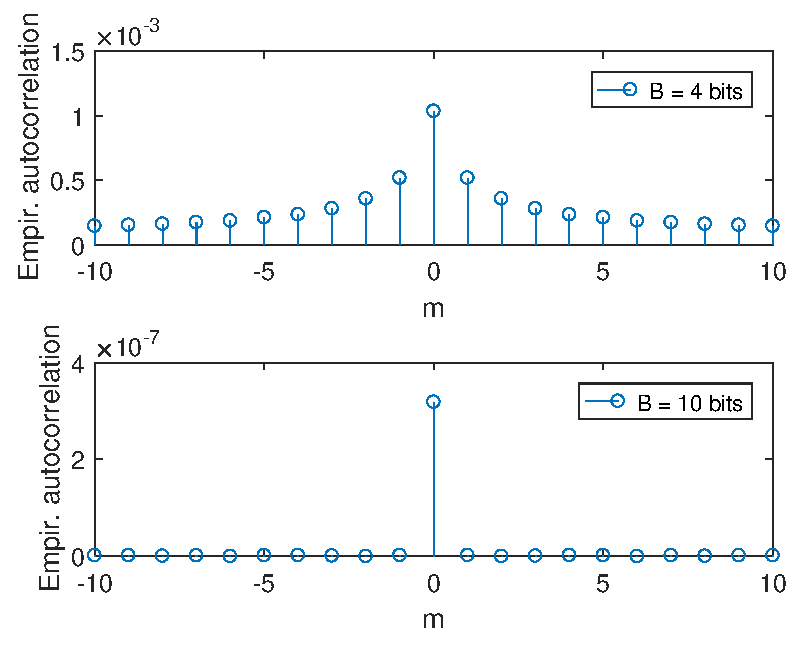
\includegraphics[scale=0.7]{figs/hw03_q4_empir_xcorr.eps}
	\caption{Empirical autocorrelation functions for $B = 4$ and $B = 10$ bits.}
\end{figure}

The average power is simply the autocorrelation function evaluated at 0. Therefore, we have:

\begin{align*}
\hat{\sigma}_e^2 = \begin{cases}
0.001, & B = 4~\text{bits} \\
3.1841\times 10^{-7}, & B = 10~\text{bits} \\
\end{cases}
\end{align*}

Recall that as discussed in class, by assuming quantization noise as an uniformly distributed noise: $\sigma_e^2 = \Delta^2/12$. For each case,
\begin{align*}
\sigma_e^2 = \begin{cases}
0.0013, & B = 4~\text{bits} \\
3.1789\times 10^{-7}, & B = 10~\text{bits} \\
\end{cases}
\end{align*}

Note that these estimates are very accurate even when quantization is coarse. 

\noindent\textbf{Part 2: Noise shaping without oversampling}
\subsection{(c)}

The code for part (c) is included on the next page.

\noindent\textbf{Part 3: Noise shaping with oversampling}
\subsection{(d)}

The code for part (d) is included on the next page.

\subsection{(e)}

The code for part (e) is included on the next page.

The noise power after noise shaping and filtering is $\tilde{\sigma}_e^2 = 1.113\times 10^{-4}$. We can define the signal-to-noise ratio (SNR) improvement 
\begin{equation}
\text{SNR}_{\text{improvement}} = 10\log_{10}\Big(\frac{\tilde{\sigma}_e^2}{\sigma_e^2}\Big) = 9.6858~\text{dB (or 9.3021 in linear units)}.
\end{equation}

Since for every extra bit of resolution we have a 6.02 dB improvement of SNR. This improvement in SNR would be equivalent to increase the quantizer resolution by 1.6 bits. More significant improvements could be achieved either by using higher oversampling factor $M$ or higher-order noise shaping (different filter $H(z)$).
\subsection{Matlab code for parts (b) through (e)}
% This file was automatically created from the m-file 
% "m2tex.m" written by USL. 
% The fontencoding in this file is UTF-8. 
%  
% You will need to include the following two packages in 
% your LaTeX-Main-File. 
%  
% \usepackage{color} 
% \usepackage{fancyvrb} 
%  
% It is advised to use the following option for Inputenc 
% \usepackage[utf8]{inputenc} 
%  
  
% definition of matlab colors: 
\definecolor{mblue}{rgb}{0,0,1} 
\definecolor{mgreen}{rgb}{0.13333,0.5451,0.13333} 
\definecolor{mred}{rgb}{0.62745,0.12549,0.94118} 
\definecolor{mgrey}{rgb}{0.5,0.5,0.5} 
\definecolor{mdarkgrey}{rgb}{0.25,0.25,0.25} 
  
\DefineShortVerb[fontfamily=courier,fontseries=m]{\$} 
\DefineShortVerb[fontfamily=courier,fontseries=b]{\#} 
  
\noindent                                                                              
 \hspace*{-1.6em}{\scriptsize 1}$  $\color{mgrey}#%% Template for Homework 3: Problem 3 on quantization and quantization noise shaping#\color{black}$$\\
 \hspace*{-1.6em}{\scriptsize 2}$  clear, $\color{mdarkgrey}$clc, close all $\color{black}$$\color{mgrey}$% clear variables$\color{black}$$\\
 \hspace*{-1.6em}{\scriptsize 3}$  $\\
 \hspace*{-1.6em}{\scriptsize 4}$  $\color{mgrey}$% Load speech signal$\color{black}$$\\
 \hspace*{-1.6em}{\scriptsize 5}$  [x, Fs] = audioread($\color{mdarkgrey}$'speech_dft.wav'$\color{black}$);          $\color{mgrey}$% Fs is sampling frequency$\color{black}$$\\
 \hspace*{-1.6em}{\scriptsize 6}$  T = 1/Fs;                                       $\color{mgrey}$% sampling period$\color{black}$$\\
 \hspace*{-1.6em}{\scriptsize 7}$  $\\
 \hspace*{-1.6em}{\scriptsize 8}$  $\color{mgrey}#%% Important: #\color{black}$$\\
 \hspace*{-1.6em}{\scriptsize 9}$  $\color{mgrey}$% If your simulations take too long because you're using a slow computer,$\color{black}$$\\
 \hspace*{-2em}{\scriptsize 10}$  $\color{mgrey}$% you can uncomment the following line in order to use just part of the $\color{black}$$\\
 \hspace*{-2em}{\scriptsize 11}$  $\color{mgrey}$% speech signal. Specifically, you may use just the first 43000 samples, $\color{black}$$\\
 \hspace*{-2em}{\scriptsize 12}$  $\color{mgrey}$% which correspond to the phrase "The discrete Fourier transform". $\color{black}$$\\
 \hspace*{-2em}{\scriptsize 13}$  $\color{mgrey}$% In my computer, the simulations with the whole signal took < 1 s.$\color{black}$$\\
 \hspace*{-2em}{\scriptsize 14}$  $\color{mgrey}$% x = x(1:43e3); % play just part of the speech$\color{black}$$\\
 \hspace*{-2em}{\scriptsize 15}$  $\\
 \hspace*{-2em}{\scriptsize 16}$  $\color{mgrey}#%% Your code goes here#\color{black}$$\\
 \hspace*{-2em}{\scriptsize 17}$  $\color{mgrey}$%sound(x, Fs) % Play speech$\color{black}$$\\
 \hspace*{-2em}{\scriptsize 18}$  $\\
 \hspace*{-2em}{\scriptsize 19}$  $\color{mgrey}$% Define parameters$\color{black}$$\\
 \hspace*{-2em}{\scriptsize 20}$  range_lims = [-1 1];           $\color{mgrey}$% range limits                  $\color{black}$$\\
 \hspace*{-2em}{\scriptsize 21}$  B = 4; $\color{mgrey}$% quantizer resolution$\color{black}$$\\
 \hspace*{-2em}{\scriptsize 22}$  $\\
 \hspace*{-2em}{\scriptsize 23}$  $\color{mgrey}#%% Part (b)#\color{black}$$\\
 \hspace*{-2em}{\scriptsize 24}$  maxLag = 10;$\\
 \hspace*{-2em}{\scriptsize 25}$  [~, $\color{mdarkgrey}$e4bits] = quantizer(x, 4, range_lims); $\color{black}$$\\
 \hspace*{-2em}{\scriptsize 26}$  [~, $\color{mdarkgrey}$e10bits] = quantizer(x, 10, range_lims); $\color{black}$$\\
 \hspace*{-2em}{\scriptsize 27}$  $\\
 \hspace*{-2em}{\scriptsize 28}$  c4bits = xcorr(e4bits, e4bits, maxLag, $\color{mdarkgrey}$'unbiased'$\color{black}$);$\\
 \hspace*{-2em}{\scriptsize 29}$  c10bits = xcorr(e10bits, e10bits, maxLag, $\color{mdarkgrey}$'unbiased'$\color{black}$);$\\
 \hspace*{-2em}{\scriptsize 30}$  $\\
 \hspace*{-2em}{\scriptsize 31}$  e4bits_power = c4bits(maxLag+1); $\color{mgrey}$% autocorrelation at m = 0;$\color{black}$$\\
 \hspace*{-2em}{\scriptsize 32}$  e10bits_power = c10bits(maxLag+1); $\color{mgrey}$% autocorrelation at m = 0;$\color{black}$$\\
 \hspace*{-2em}{\scriptsize 33}$  $\\
 \hspace*{-2em}{\scriptsize 34}$  $\color{mgrey}$% Plot autocorrelation function$\color{black}$$\\
 \hspace*{-2em}{\scriptsize 35}$  figure, $\color{mdarkgrey}$subplot(211), box on$\color{black}$$\\
 \hspace*{-2em}{\scriptsize 36}$  stem(-maxLag:maxLag, $\color{mdarkgrey}$c4bits)$\color{black}$$\\
 \hspace*{-2em}{\scriptsize 37}$  legend($\color{mdarkgrey}$'B = 4 bits'$\color{black}$)$\\
 \hspace*{-2em}{\scriptsize 38}$  xlabel($\color{mdarkgrey}$'m'$\color{black}$, $\color{mdarkgrey}$'FontSize'$\color{black}$, 12)$\\
 \hspace*{-2em}{\scriptsize 39}$  ylabel($\color{mdarkgrey}$'Empir. autocorrelation'$\color{black}$, $\color{mdarkgrey}$'FontSize'$\color{black}$, 12)$\\
 \hspace*{-2em}{\scriptsize 40}$  set(gca, $\color{mdarkgrey}$'FontSize'$\color{black}$, 12)$\\
 \hspace*{-2em}{\scriptsize 41}$  subplot(212), $\color{mdarkgrey}$box on$\color{black}$$\\
 \hspace*{-2em}{\scriptsize 42}$  stem(-maxLag:maxLag, $\color{mdarkgrey}$c10bits)$\color{black}$$\\
 \hspace*{-2em}{\scriptsize 43}$  legend($\color{mdarkgrey}$'B = 10 bits'$\color{black}$)$\\
 \hspace*{-2em}{\scriptsize 44}$  xlabel($\color{mdarkgrey}$'m'$\color{black}$, $\color{mdarkgrey}$'FontSize'$\color{black}$, 12)$\\
 \hspace*{-2em}{\scriptsize 45}$  ylabel($\color{mdarkgrey}$'Empir. autocorrelation'$\color{black}$, $\color{mdarkgrey}$'FontSize'$\color{black}$, 12)$\\
 \hspace*{-2em}{\scriptsize 46}$  set(gca, $\color{mdarkgrey}$'FontSize'$\color{black}$, 12)$\\
 \hspace*{-2em}{\scriptsize 47}$  saveas(gca, $\color{mdarkgrey}$'../figs/hw03_q4_empir_xcorr'$\color{black}$, $\color{mdarkgrey}$'epsc'$\color{black}$)$\\
 \hspace*{-2em}{\scriptsize 48}$  $\\
 \hspace*{-2em}{\scriptsize 49}$  $\color{mgrey}#%% Part (c)#\color{black}$$\\
 \hspace*{-2em}{\scriptsize 50}$  B = 4; $\color{mgrey}$% quantizer resolution$\color{black}$$\\
 \hspace*{-2em}{\scriptsize 51}$  b = [1 -1]; $\color{mgrey}$% shaping filter coefficients$\color{black}$$\\
 \hspace*{-2em}{\scriptsize 52}$  $\\
 \hspace*{-2em}{\scriptsize 53}$  [xq, $\color{mdarkgrey}$e] = quantizer(x, B, range_lims); $\color{black}$$\\
 \hspace*{-2em}{\scriptsize 54}$  $\\
 \hspace*{-2em}{\scriptsize 55}$  eshaped = filter(b, 1, e);$\\
 \hspace*{-2em}{\scriptsize 56}$  $\\
 \hspace*{-2em}{\scriptsize 57}$  xqshaped = x + eshaped;$\\
 \hspace*{-2em}{\scriptsize 58}$  $\color{mgrey}$%sound(xqshaped, Fs)$\color{black}$$\\
 \hspace*{-2em}{\scriptsize 59}$  $\\
 \hspace*{-2em}{\scriptsize 60}$  $\color{mgrey}#%% Part (d)#\color{black}$$\\
 \hspace*{-2em}{\scriptsize 61}$  B = 4; $\color{mgrey}$% quantizer resolution$\color{black}$$\\
 \hspace*{-2em}{\scriptsize 62}$  b = [1 -1]; $\color{mgrey}$% shaping filter coefficients$\color{black}$$\\
 \hspace*{-2em}{\scriptsize 63}$  M = 3; $\color{mgrey}$% upsampling factor $\color{black}$$\\
 \hspace*{-2em}{\scriptsize 64}$  [xq, $\color{mdarkgrey}$e] = quantizer(x, B, range_lims); $\color{black}$$\\
 \hspace*{-2em}{\scriptsize 65}$  $\\
 \hspace*{-2em}{\scriptsize 66}$  eup = upsample(e, M);$\\
 \hspace*{-2em}{\scriptsize 67}$  eshaped = filter(b, 1, eup);$\\
 \hspace*{-2em}{\scriptsize 68}$  ef = M*decimate(eshaped, M); $\color{mgrey}$% Note multiplication by M in order to account $\color{black}$$\\
 \hspace*{-2em}{\scriptsize 69}$  $\color{mgrey}$% for the fact that in Fig. 6a the signal is also decimated$\color{black}$$\\
 \hspace*{-2em}{\scriptsize 70}$  $\\
 \hspace*{-2em}{\scriptsize 71}$  xqshaped = x + ef;$\\
 \hspace*{-2em}{\scriptsize 72}$  sound(xqshaped, $\color{mdarkgrey}$Fs)$\color{black}$$\\
 \hspace*{-2em}{\scriptsize 73}$  $\\
 \hspace*{-2em}{\scriptsize 74}$  ef_power = mean(abs(ef).^2); $\color{mgrey}$% can use var only if ef is zero mean$\color{black}$$\\
 \hspace*{-2em}{\scriptsize 75}$  $\\
 \hspace*{-2em}{\scriptsize 76}$  SNRimprovement = 10*log10(e4bits_power/ef_power)$\\
 \hspace*{-2em}{\scriptsize 77}$  $\\
 \hspace*{-2em}{\scriptsize 78}$  Bimprovement = SNRimprovement/6.02$\\ 
  
\UndefineShortVerb{\$} 
\UndefineShortVerb{\#}

\end{document}